\section{1174003 - Dwi Septiani Tsaniyah}
\subsection{Teori}
\begin{enumerate}
	\item Sejarah dan Perkembangan
	\hfill\break
	Kecerdasan buatan adalah bidang ilmu komputer yang sangat penting di masa kini dan masa depan untuk mewujudkan sistem komputer cerdas. "Intelligo" yang berarti "Saya mengerti". Berarti dasar kecerdasan untuk mengatasi dan mengambil tindakan. Sebenarnya, bidang Artificial Intelligence, atau disingkat AI, yang diambil dari tampilan komputer sekitar tahun 1940-an, sedangkan sejarah perkembangannya dapat ditelusuri sejak zaman Mesir kuno. Pada saat ini, perhatian diberikan pada kemampuan komputer untuk melakukan hal-hal yang dapat dilakukan manusia. Dalam hal ini, komputer dapat menggunakan kecerdasan dan komunikasi manusia McMulloh dan Pitts pada tahun 1943 meminta model matematika yang disebut perceptron neuron di otak. Mereka juga menunjukkan bagaimana neuron menjadi aktif seperti sakelar on-off dan neuron dapat belajar dan memberikan tindakan yang berbeda dari input yang diberikan. Kontribusi terbesar dalam bidang AI dimulai dengan karya Alan Turing, pada tahun 1950 yang mencoba menjawab "Can computer think" dengan menciptakan mesin Turing. Makalah Alan Turing tahun 1950 berjudul "Mesin Komputer dan Kecerdasan" membahas istilah-istilah mesin yang dianggap cerdas. Dia berasumsi bahwa jika sebuah mesin dapat berhasil berperilaku seperti manusia, kita dapat menganggapnya sebagai kecerdasan. Ada 3 faktor utama yang menyebabkan hal itu terjadi:
	\begin{itemize}
		\item Banyak subjek pada program AI yang bermunculan hanya mengandung sedikit atau bahkan sama sekali tidak  mengandung sama sekali pengetahuan (knowledge).
		\item Kecerdasan buatan harus bisa menyelesaikan banyak masalah.
		\item Untuk menghasilkan perilkau intelijensia ada beberapa batasan pada struktur yang bisa digunakan.
	\end{itemize}
	Definisi kecerdasan buatan itu sendiri adalah suatu system teknologi yang didalamnya ditambahakan kecerdasan oleh manusia, kecerdasan buatan diatur dan dikembangkan dalam konteks ilmiah, dan bentukan dari kecerdasan entitas ilmiah yang ada.
	\item Definisi
	\hfill\break
	Supervised learning, klasifikasi, regresi, unsupervised learning, dataset, trainingset dan testingset.
	\begin{itemize}
		\item Supervised Learning
		\hfill\break
		Supervised Learning merupakan sebuah tipe learning yang mempunyai variable input dan variable output, tipe ini juga menggunakan satu algoritma atau lebih dari satu algoritma yang digunakan untuk mempelajari fungsi  pemetaan dari input ke output.
		\item Klasifikasi
		\hfill\break
		Klasifikasi adalah pengelompokan data di mana data yang digunakan memiliki label atau kelas target. Sehingga algoritma untuk menyelesaikan masalah klasifikasi dikategorikan ke dalam pembelajaran terbimbing.
		\item Regresi
		\hfill\break
		regressi metode analisis statistik yang digunakan untuk dapat melihat efek antara dua atau lebih variabel. Hubungan variabel dalam pertanyaan adalah fungsional yang diwujudkan dalam bentuk model matematika. Dalam analisis regresi, variabel dibagi menjadi dua jenis, yaitu variabel respons atau yang biasa disebut variabel dependen dan variabel independen atau dikenal sebagai variabel independen. Ada beberapa jenis analisis regresi, yaitu regresi sederhana yang mencakup linear sederhana dan regresi non-linear sederhana dan regresi berganda yang mencakup banyak linier atau non-linear berganda. Analisis regresi digunakan dalam pembelajaran mesin pembelajaran dengan metode pembelajaran terawasi.
		\item Unsupervised learning 
		\hfill\break
		unsupervised learning jenis pembelajaran di mana kita hanya memiliki data input (input data) tetapi tidak ada variabel output yang terkait. Tujuan dari pembelajaran tanpa pengawasan adalah untuk memodelkan struktur dasar atau distribusi data dengan tujuan mempelajari data lebih lanjut, dengan kata lain, itu adalah fungsi simpulan yang menggambarkan atau menjelaskan data.
		\item Data set
		\hfill\break
		Data set objek yang merepresentasikan data dan relasinya di memory. Strukturnya mirip dengan data di database. Dataset berisi koleksi dari datatable dan datarelation.
		\item Training Set
		\hfill\break
		Training set adalah bagian dari dataset yang di latih untuk membuat prediksi atau menjalankan fungsi dari algoritma ML lain sesuai dengan masing-masing. Memberikan instruksi melalui algoritma sehingga mesin yang di praktikkan dapat menemukan korelasinya sendiri.
		\item Testing Set
		\hfill\break
		testing set adalah bagian dari dataset yang kami uji untuk melihat akurasinya, atau dengan kata lain untuk melihat kinerjanya.
	\end{itemize}
\end{enumerate}
\subsection{Praktek}
\begin{enumerate}
	\item Instalasi Library scikit dari ianaconda, mencoba kompilasi dan uji coba ambil contoh kode dan lihat variabel explorer
	\hfill\break
	\begin{figure}[H]
		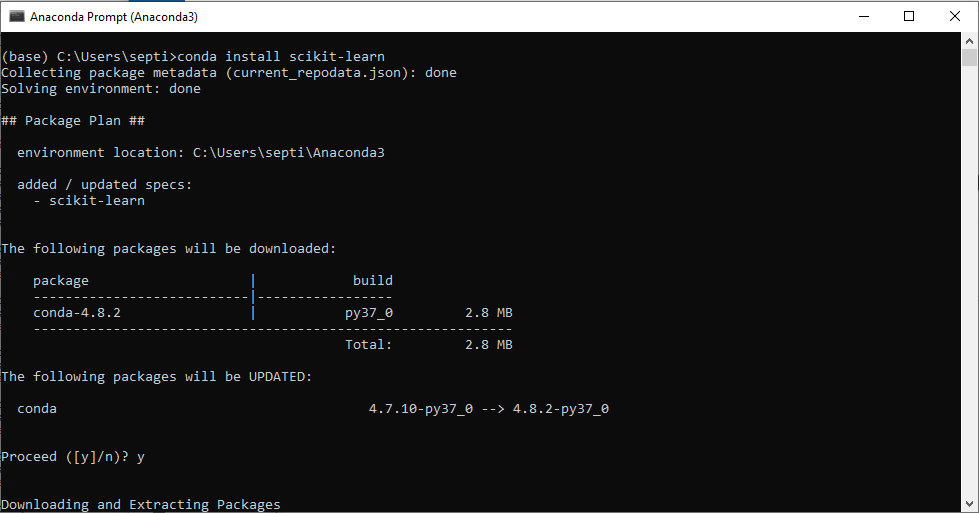
\includegraphics[width=4cm]{figures/1174003/1/1.PNG}
		\centering
		\caption{Instalasi Package Scikit Learn}
	\end{figure}
	\begin{figure}[H]
		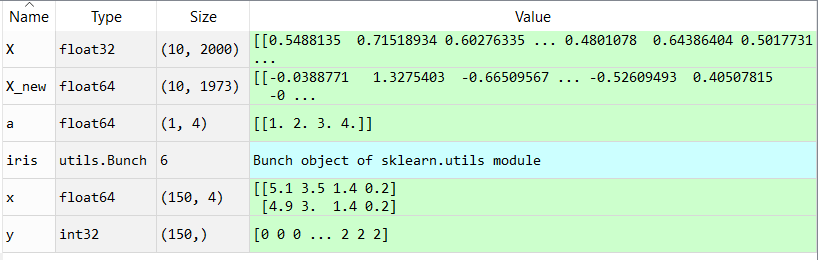
\includegraphics[width=4cm]{figures/1174003/1/2.PNG}
		\centering
		\caption{Isi Variabel Explorer}
	\end{figure}
	\item Mencoba loading an example dataset
	\hfill\break
	\lstinputlisting[firstline=8, lastline=12]{src/1174003/1/1174003.py}
	\item Mencoba Learning dan predicting
	\hfill\break
	\lstinputlisting[firstline=14, lastline=24]{src/1174003/1/1174003.py}
	\item Mencoba Model Persistence
	\hfill\break
	\lstinputlisting[firstline=26, lastline=36]{src/1174003/1/1174003.py}
	\item Mencoba Conventions
	\hfill\break
	\lstinputlisting[firstline=38, lastline=50]{src/1174003/1/1174003.py}
\end{enumerate}
\subsection{Penanganan Error}
\begin{enumerate}
	\item ScreenShoot Error
	\begin{figure}[H]
		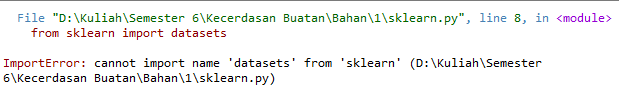
\includegraphics[width=4cm]{figures/1174031/1/error/1.png}
		\centering
		\caption{Import Error}
	\end{figure}
	\begin{figure}[H]
		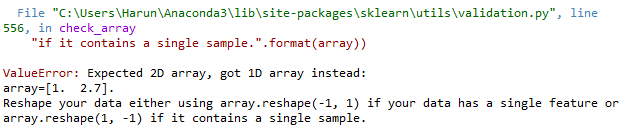
\includegraphics[width=4cm]{figures/1174031/1/error/2.png}
		\centering
		\caption{Value Error}
	\end{figure}
	\item Tuliskan Kode Error dan Jenis Error
	\begin{itemize}
		\item Import Error
		\item Value Error
	\end{itemize}
	\item Cara Penangan Error
	\begin{itemize}
		\item Import Error
		\hfill\break
		Dengan Menginstall Library Yang Tidak Ditemukan
		\item Value Error
		\hfill\break
		Mengubah Bentuk Arraynya, Menjadi 1 Dimensi
	\end{itemize}
\end{enumerate}
\subsection{Bukti Tidak Plagiat}
\begin{figure}[H]
	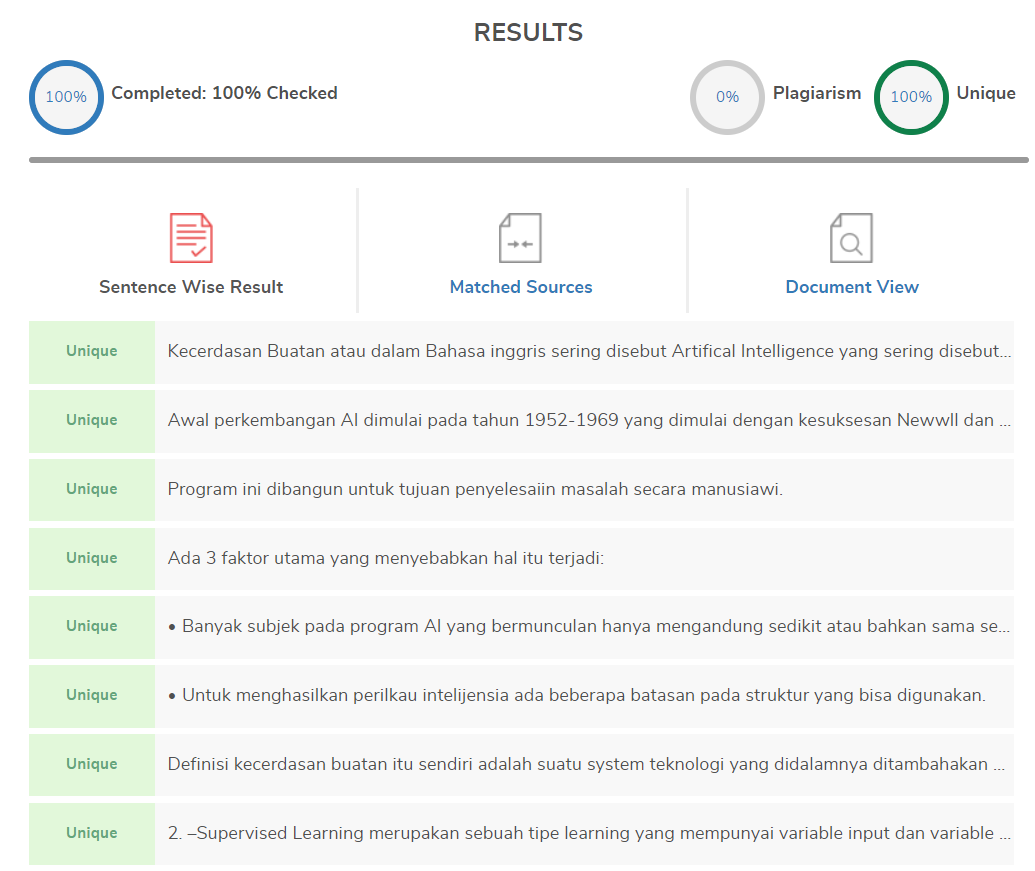
\includegraphics[width=4cm]{figures/1174031/1/plagiat/1.PNG}
	\centering
	\caption{Bukti Tidak Melakukan Plagiat 1}
\end{figure}